%!TEX root = ../paper.tex

\begin{figure}
	\centering
	\begin{subfigure}{0.23\textwidth}
		\centering
		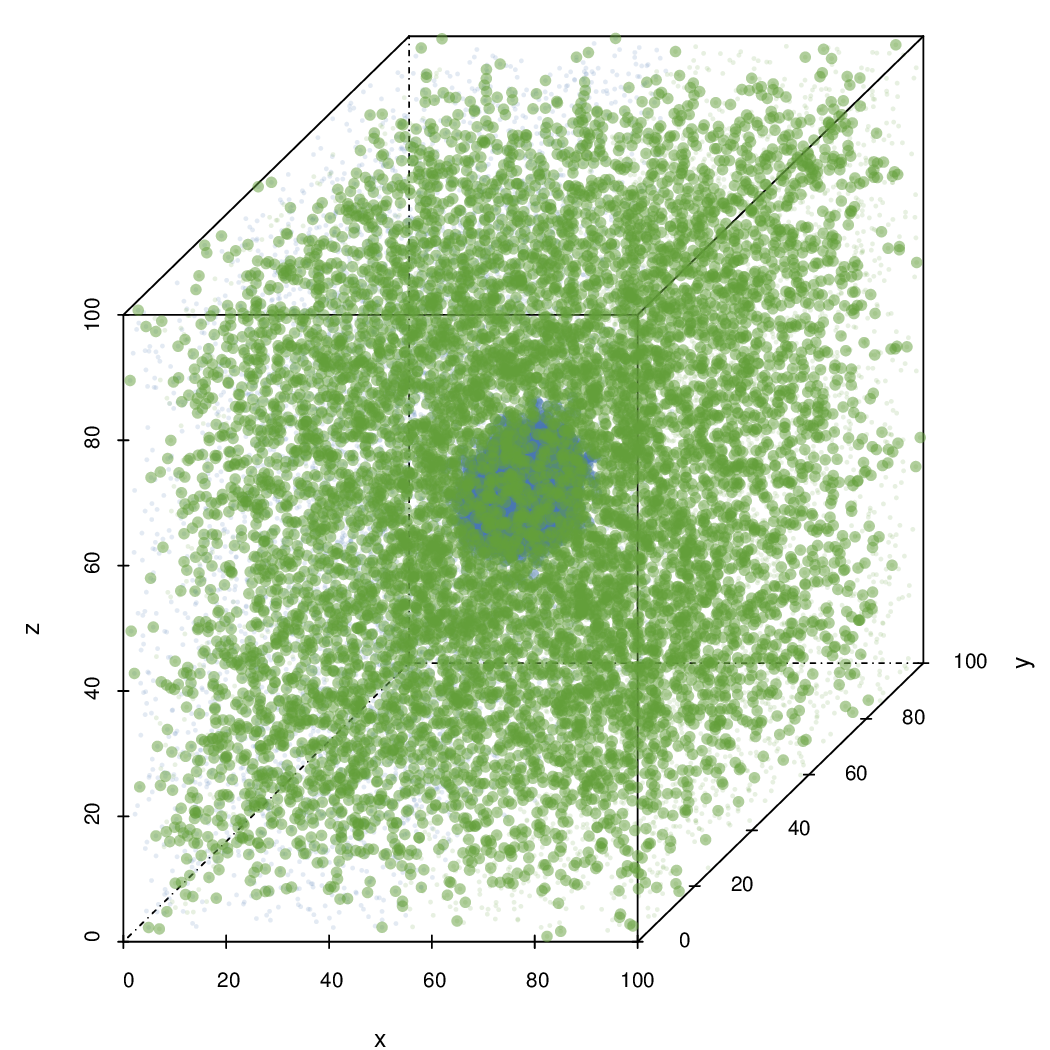
\includegraphics[keepaspectratio=true, width=\textwidth, height=0.23\textheight]{discussion/img/ferdosi_1_abs_error_mbeSmallerThansambe}
		\caption{Dataset \ferdosiOne}
		\label{fig:discussion:singleSphere:mbeLowerError:ferdosi1}
	\end{subfigure}
	\begin{subfigure}{0.23\textwidth}
		\centering
		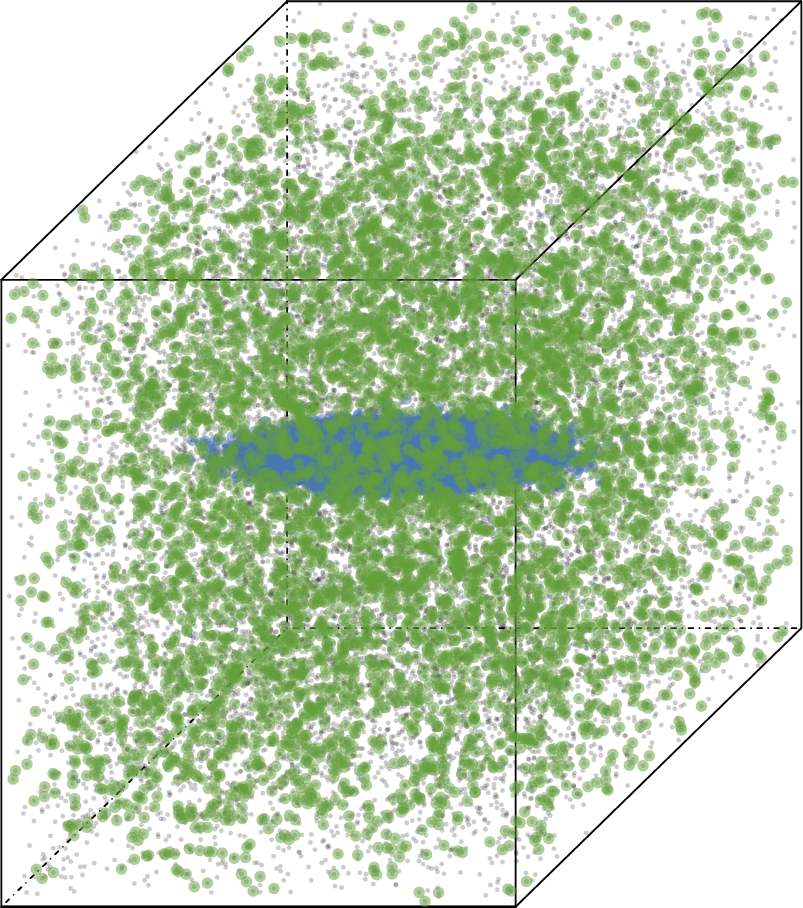
\includegraphics[keepaspectratio=true, width=\textwidth, height=0.23\textheight]{discussion/img/baakman_1_abs_error_mbeSmallerThansambe}
		\caption{Dataset \baakmanOne}
		\label{fig:discussion:singleSphere:mbeLowerError:baakman1}
	\end{subfigure}	
	\begin{subfigure}{0.23\textwidth}
		\centering
		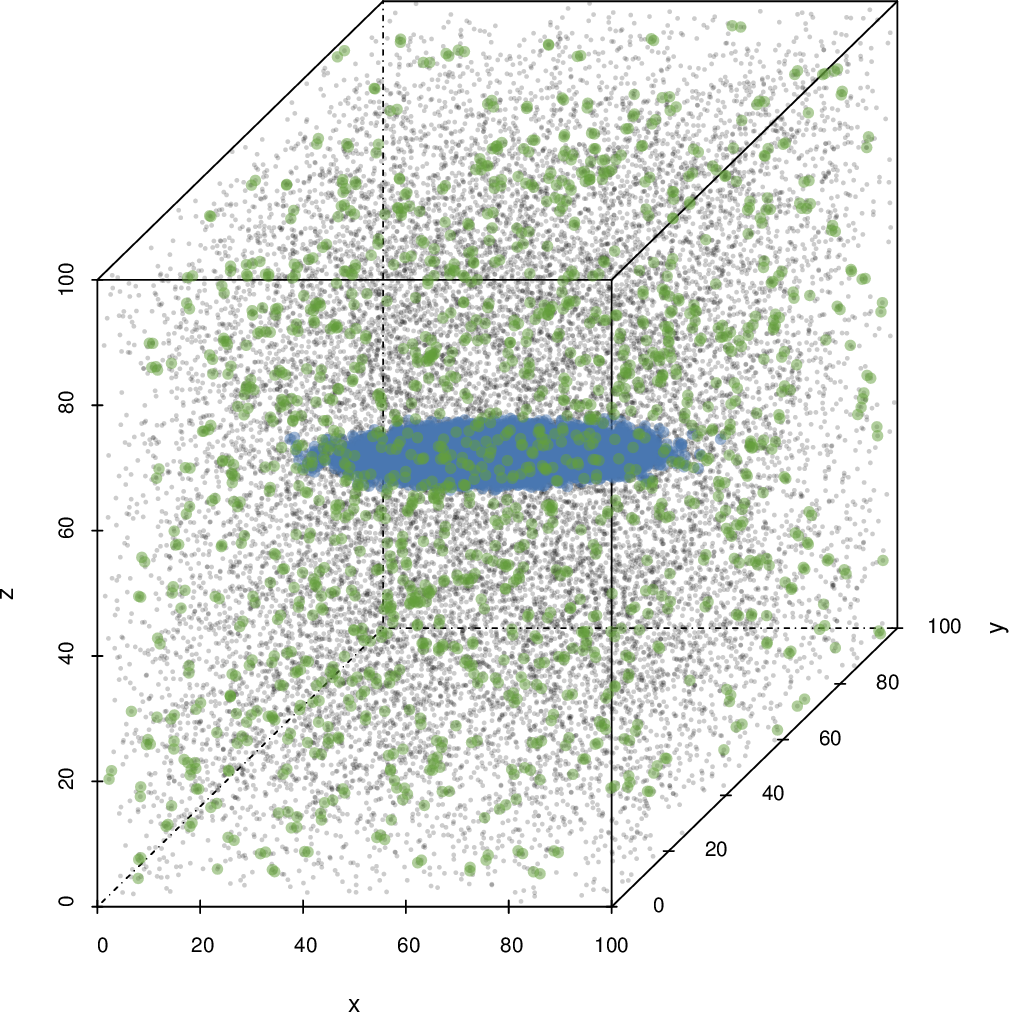
\includegraphics[keepaspectratio=true, width=\textwidth, height=0.23\textheight]{discussion/img/baakman_4_abs_error_mbeSmallerThansambe}
		\caption{Dataset \baakmanFour}
		\label{fig:discussion:singleSphere:mbeLowerError:baakman4}
	\end{subfigure}		
	\begin{subfigure}{0.23\textwidth}
		\centering
		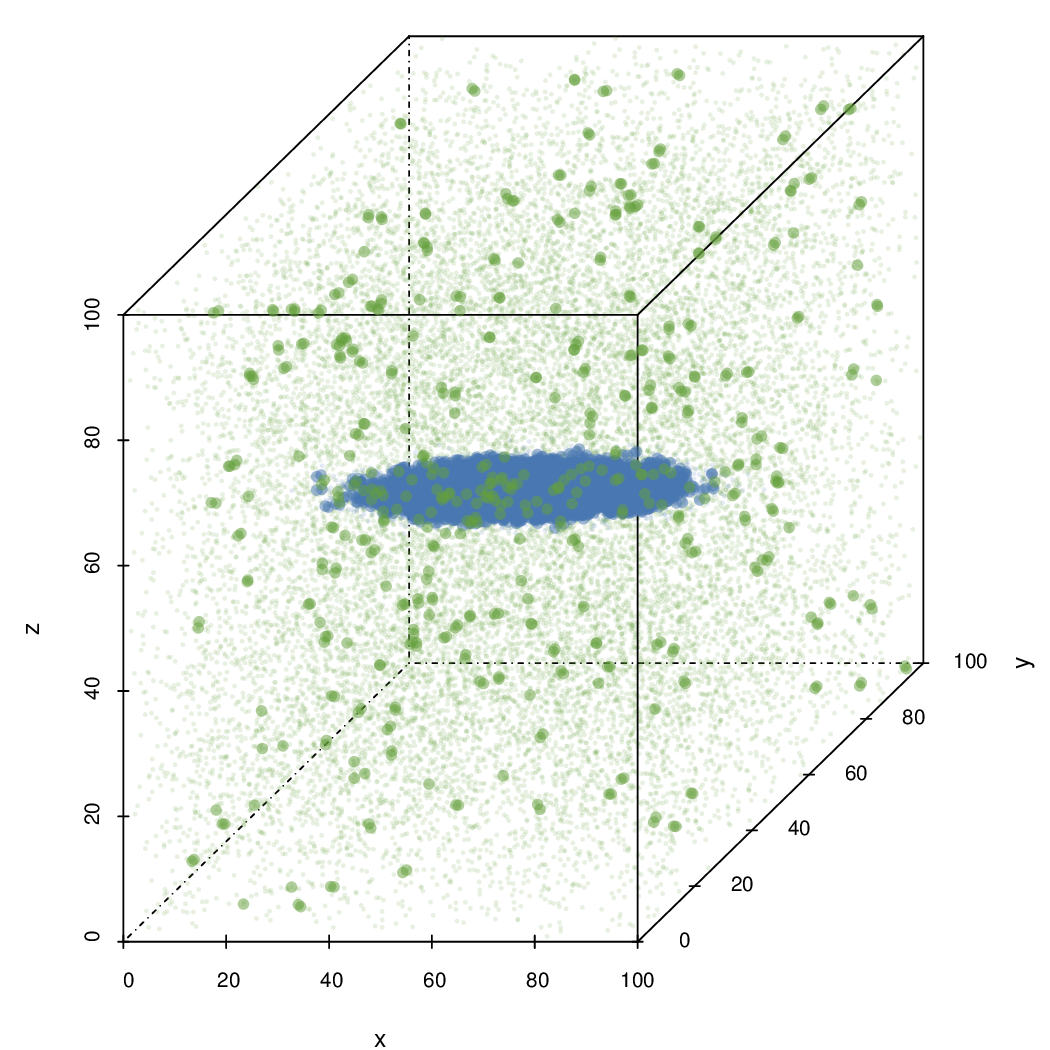
\includegraphics[keepaspectratio=true, width=\textwidth, height=0.23\textheight]{discussion/img/baakman_5_abs_error_mbeSmallerThansambe}
		\caption{Dataset \baakmanFive}
		\label{fig:discussion:singleSphere:mbeLowerError:baakman5}
	\end{subfigure}			
	\caption{Low opacity scatter plot of dataset %
		\subref{fig:discussion:singleSphere:mbeLowerError:ferdosi1} \ferdosiOne, %
		\subref{fig:discussion:singleSphere:mbeLowerError:baakman1} \baakmanOne, %
		\subref{fig:discussion:singleSphere:mbeLowerError:baakman4} \baakmanFour, and%
		\subref{fig:discussion:singleSphere:mbeLowerError:baakman5} \baakmanFive, %
		with an overlay of larger points with a higher opacity where the absolute error of \sambe is larger than or equal to the absolute error of \mbe.}
	\label{fig:discussion:singleSphere:mbeLowerError}
\end{figure}

% Introduction
The scatter plots of the datasets with a single Gaussian in \cref{fig:discussion:singleSphere:mbeLowerError} emphasize the points where the absolute error of the symmetric estimator is smaller than that of the shape-adaptive estimator. 

	% Ferdosi 1
		% ALl POINTS
		% SAMBE better than MBE: 2.828800000000000e+04 (4.727588742563005e+01 percent)
		% MBE better than SAMBE: 3.154800000000000e+04 (5.272411257436994e+01 percent)
		% MBE equal to SAMBE: 0.000000000000000e+00 (0.000000000000000e+00 percent)
		
		% Component 0
		% MSE(MBE, SAMBE):
		%  1.245351981191544e-08	& 1.335673957702697e-08

		% SAMBE better than MBE: 1.773700000000000e+04 (4.434250000000000e+01 percent)
		% MBE better than SAMBE: 2.226300000000000e+04 (5.565750000000001e+01 percent)
		% MBE equal to SAMBE: 0.000000000000000e+00 (0.000000000000000e+00 percent)

		% Component 1
		% MSE(MBE, SAMBE):
		%  1.046361645486837e-11	& 1.282383835662826e-11

		% SAMBE better than MBE: 1.055100000000000e+04 (5.319116757410768e+01 percent)
		% MBE better than SAMBE: 9.285000000000000e+03 (4.680883242589232e+01 percent)
		% MBE equal to SAMBE: 0.000000000000000e+00 (0.000000000000000e+00 percent)	


		% The overlay plot
		\Cref{fig:discussion:singleSphere:mbeLowerError:ferdosi1} shows that the shape-adaptive estimator results outperforms the symmetric estimators on most points near the boundary of the dataset. It also seems to illustrate that that \mbe results in a lower error than \sambe on the other points, however the raw data shows that on \num{5.272411257436994e+01}\% of the full dataset, and on \num{5.565750000000001e+01} \% of the Gaussian component the symmetric estimator results in a lower absolute error.
		% The shape of the kernels
		Reviewing the shape of the kernels used for the points in dataset \ferdosiOne we find that the used kernels are all near spherical. The kernels with the largest differences between their eigenvalues are associated with points near the boundary of the dataset. 
		% Largest differnces in estimated values between kernels. 
		The largest differences in error between the two estimators can be found near the center of the Gaussian component, where the shape-adaptive kernels are relatively spherical. The difference between the two estimators at these points is caused by the number of points used to estimate the density, for most of these points \sambe uses too many points which results in an overestimated density. 

	% Baakman 1
		% Component -1
		% MSE(MBE, SAMBE):
		%  1.494313211797496e-08	& 1.544094229246398e-08
		% SAMBE better than MBE: 2.509400000000000e+04 (4.193796376763152e+01 percent)
		% MBE better than SAMBE: 2.680000000000000e+04 (4.478909017982485e+01 percent)
		% MBE equal to SAMBE: 7.942000000000000e+03 (1.327294605254362e+01 percent)

		% Component 0
		% MSE(MBE, SAMBE):
		%  2.231981590358483e-08	& 2.306388047782812e-08
		% SAMBE better than MBE: 1.924800000000000e+04 (4.812000000000000e+01 percent)
		% MBE better than SAMBE: 2.061300000000000e+04 (5.153250000000001e+01 percent)
		% MBE equal to SAMBE: 1.390000000000000e+02 (3.475000000000000e-01 percent)

		% Component 1
		% MSE(MBE, SAMBE):
		%  6.778671444628963e-11	& 6.901612718035766e-11
		% SAMBE better than MBE: 5.846000000000000e+03 (2.947166767493447e+01 percent)
		% MBE better than SAMBE: 6.187000000000000e+03 (3.119076426698931e+01 percent)
		% MBE equal to SAMBE: 7.803000000000000e+03 (3.933756805807623e+01 percent)

		% Overlay plot
		The results in \cref{fig:discussion:singleSphere:mbeLowerError:baakman1} are comparable to those in \cref{fig:experiment:singlesphere:ferdosi1}, however there seem to be fewer points of the noise component where the absolute error of using the symmetric-kernel is lower than using a shape-adaptive kernel. Reviewing the raw data shows that this difference is primarily caused by the \num{7.803000000000000e+03} points for which both estimators estimate the same density. Due to the elongated shape of the distribution its shape influences the kernel of fewer shapes of the noise component resulting in more spherical kernels, which results in the same density estimate for a larger number of points. 
		% The shape of the kernels
		As in dataset \ferdosiOne the points with the most ellipsoidal kernels are positioned near the boundaries of the dataset, where \sambe outperforms \mbe. 
		% Largest differences in estiamted values between estimators
		The points whose differences in estimated densities are largest are, as in dataset \ferdosiOne, found near the mean of the Gaussian distribution. At first this seems counterintuitive since the kernels are relatively spherical near the Gaussian component, however we expect that due to the high density of points in that area a small change to the shape of the kernel has a large effect. This is confirmed by the large differences in the number of patterns that are used in the density estimate of the points near the mean of the Gaussian component between the two estimators. 

	%Baakman 4
		% Component -1
		% MSE(MBE, SAMBE):
		%  2.945143538188240e-08	& 2.971553835946330e-08

		% SAMBE better than MBE: 2.061700000000000e+04 (3.445584597900929e+01 percent)
		% MBE better than SAMBE: 2.132900000000000e+04 (3.564576509124942e+01 percent)
		% MBE equal to SAMBE: 1.789000000000000e+04 (2.989838892974129e+01 percent)	
		% Component 0
		% MSE(MBE, SAMBE):
		%  4.404296246131644e-08	& 4.443607459199309e-08

		% SAMBE better than MBE: 1.926500000000000e+04 (4.816250000000000e+01 percent)
		% MBE better than SAMBE: 1.988200000000000e+04 (4.970500000000000e+01 percent)
		% MBE equal to SAMBE: 8.530000000000000e+02 (2.132500000000000e+00 percent)


		% Component 1
		% MSE(MBE, SAMBE):
		%  2.710168671393879e-11	& 3.105311540244085e-11

		% SAMBE better than MBE: 1.352000000000000e+03 (6.815890300463804e+00 percent)
		% MBE better than SAMBE: 1.447000000000000e+03 (7.294817503528937e+00 percent)
		% MBE equal to SAMBE: 1.703700000000000e+04 (8.588929219600726e+01 percent)	
	
		% Overlay Plot
		In \cref{fig:discussion:singleSphere:mbeLowerError:baakman4} we observe that the \mbe outperforms \sambe on very few points in dataset \baakmanFour, to be exact on \num{92.7051824965} percent of the points the absolute error of the shape-adaptive estimator was at least as low as the error of the symmetric estimator. Once again we attribute this difference in performance to the elongated shape of the Gaussian component. 
		% Shape of the kernels
		Reviewing the shape of the kernel we find kernels with a strongly adapted shape both near the boundary of the dataset, where \sambe outperforms \mbe, and near the Gaussian component.
		% Largest differences in estimated values between estimators
		Near the mean of this component we also find the biggest differences in estimated densities between the two estimators. 

	%Baakman 5
		% Component -1
		% MSE(MBE, SAMBE):
		%  5.587052323057813e-08	& 5.600040277292591e-08

		% SAMBE better than MBE: 1.935100000000000e+04 (3.234006283842503e+01 percent)
		% MBE better than SAMBE: 1.933100000000000e+04 (3.230663814426098e+01 percent)
		% MBE equal to SAMBE: 2.115400000000000e+04 (3.535329901731399e+01 percent)

		% Component 0
		% MSE(MBE, SAMBE):
		%  8.350875457323442e-08	& 8.370053660739159e-08
		% SAMBE better than MBE: 1.892300000000000e+04 (4.730750000000000e+01 percent)
		% MBE better than SAMBE: 1.884700000000000e+04 (4.711750000000000e+01 percent)
		% MBE equal to SAMBE: 2.230000000000000e+03 (5.575000000000000e+00 percent)


		% Component 1
		% MSE(MBE, SAMBE):
		%  1.370460322391959e-10	& 1.420969966289269e-10
		% SAMBE better than MBE: 4.280000000000000e+02 (2.157693083282920e+00 percent)
		% MBE better than SAMBE: 4.840000000000000e+02 (2.440008066142367e+00 percent)
		% MBE equal to SAMBE: 1.892400000000000e+04 (9.540229885057471e+01 percent)	

		% Overlay plot
		The effect of how elongated the Gaussian component is on how well the density of the noise is estimated is even strong in dataset \baakmanFive, as illustrated in \cref{fig:discussion:singleSphere:mbeLowerError:baakman5}. The density estimate of the two estimates is the same for \num{9.540229885057471e+01}\% of the points drawn from the uniform distribution, contrastingly this is only the case for \num{5.575000000000000e+00}\% of the points from the Gaussian component. 
		% Shape of the Kernels
		As in dataset \baakmanFour the shape of the kernels is most strongly influenced by the data near the boundaries of the dataset and the Gaussian component.
		% Largest differences in estimated values between estimators
		The largest differences between the result of the two estimators are, comparable to what we observed in dataset \baakmanFour, found near the mean of the Gaussian component. 

% General observations 
% Strong difference in kernel shape near the Gaussian in baakman 4 and 5
In general we have found that if the Gaussian component is strongly elongated, as in dataset \baakmanFour and \baakmanFive, the shape of the kernels near the mean of the Gaussian component is influenced, whereas the spherical and ellipsoidal Gaussian component in dataset \ferdosiOne and \baakmanOne, respectively, hardly influences the shape of the kernels of the data points near its mean. We expect that this is caused by a lower physical density of points near the means of the more spherical Gaussians. 
% Strong difference in density estimate near the mean of the Gaussian in ferdosi 1, baakman 1, baakman 4, baakman 5
In spite of this difference between the four datasets, in all datasets the difference in estimated density between the estimators is largest near the mean of the Gaussian component. We expect that this is due to the relative high density of points at this location, which causes small differences in the shapes of the kernels to have a large effect on the final density. 